\section{Sensor theory}
The race car being used for this project deploys a high number of sensors, ranging from simple voltage meters on every other battery cell through ride height sensors and all the way to complex pieces of technology like the two LiDARs. For perception of the surroundings and understanding of the state of the car, the most relevant sensors are camera, LiDARs, IMU, INS, optical sensors and ride height sensors. Some of these needs a further explanation, and this is done in the below sections.

\subsection{LiDAR}
A LiDAR (light imaging, detection, and ranging) works by sending out light and timing how long it takes for the light to return. A typical LiDAR for autonomous vehicles has a rotating mirror that it sends an array of light beams at. This means the LiDAR covers an entire section of view, both horisontally and vertically. The resolution is set by how many channels it has vertically, how often it sends and receives light and the frequency of rotation. How far it can detect is determined by the sensitivity of the receiver and the strength of the sent beam. In a formula student application the allowed strength of the emited light is limited for safety reasons, which means the only real way of extending how far you can detect is by either increasing the sensitivity of your receivers photodetector or by increasing the number of vertical and horisontal channels. The latter will allow better outlier rejection, thus increasing how far you can detect. 

\subsection{IMU}
An Inertial Measurement Unit (IMU) measures acceleration and rate of change in rotation. It typically does so in all three dimension, amounting to a total of 6 degrees of freedom (DOF). Unless you're buying extremely expensive IMU's, it is typically going to be a MEMS (microelectromechanical system) type IMU. \par MEMS IMU's measure acceleration by having a microscopic mass attached to something elastic, so it's allowed to move in one dimension. When it is influenced by an acceleration parallel to its axis of movement, it will go in that direction. How far it moves is determined by the elasticity of the material, thus giving an indirect measure of how large the magnitude of the acceleration is. The IMU measures how much the mass has moved by a capacitance that changes with the movement of the mass. This is then converted to a measure of the acceleration along this dimension. The same is then done for the two other dimensions. \\ 

The rate of change in orientation is measured by the coriolis effect, which is the effect that a mass with a velocity in a rotating frame of reference will get an acceleration perpendicular to the velocity. A mass is made to vibrate back and forth, and when the accelerometer has a rate of rotation  with an axis perpendicular to the masses back and forth movement, it will get an acceleration perpendicular to the vibration axis. This is measured the same way as for the acceleration of the IMU. Since the way the IMU measures acceleration of the mass is restricted to one dimension, measuring the three possible dimensions of rotation demand three of these vibrating masses. \\

Since these sensors are so small, a high grade one being around the size of a box of matches, they are also noisy. The IMU on the race car therefore uses a Kalman filter and two GNSS antennas to filter away as much as possible of the noise. The output is still not good enough to use as a sole source of state estimation, as it drifts too quickly.
\subsection{Optical encoder}
To measure the angle of the steering wheel and the rate of rotation of the four wheels, optical encoders are used. They work by having a light source shine through holes in a disc mounted on the rotating part, centered on the axis of rotation. On the stationary part there are photodiodes, that send out a positive bit when the light hits them. The holes on the disc are made in a special pattern, such that the pattern of bits sent out by the photodiodes makes it possible to know at what angle the disc is currently in. This pattern typically employs a grey encoding to ensure that only one bit is changed each step. \\ 

A typical optical encoder, the ones used by Revolve NTNU included, has a stated accuracy of $\pm 10$ arcseconds, which equates to around $0.0028$ degrees. This is of course only under ideal circumstances, and does not take into acount effects such as concentricity of the glass disk on its hub, concentricity of the hub’s through bore relative to the optical disk, perpendicularity of the hub relative to the plane of the optical disk, parallelism of the optical disk face with the plane of the read head, thermal effects and so on. This is however much better accuracy than what is needed for our applications, as the error stemming from the optical encoder will be dominated by other errors. This are therefore deemed adequate.

\section{Sensor setup}
\subsection{LIDARs}
On board the car are two LIDAR's (light imaging, detection, and ranging). A Velodyne VL16 with 16 vertical channels and an Ouster OS1 with 64 vertical channels. \\ 

The Velodyne has a vertical resolution of $2.0\degrees$ spread across a $360\degrees$ field of view (FOV) and a horisontal resolution of $0.1$ degrees around the horizon and going down to $0.4\degrees$ towards the limits of it's vertical FOV, which is $\pm 15\degrees$. It's range measurmenents are accurate to $\pm 3 cm$, according to the manufacturer. \\

The Ouster has a vertical and horisontal resolution of $\pm0.01$ degrees, uniformly spaced around both it's horisontal FOV of $36\degrees$  and it's vertical FOV of $\pm 16.6\degrees$. It has a range resolution of $\pm 1.2 cm$. Both the LiDARS rotates at 20 Hz. \\

The OS1 is mounted in the hoop above the driver and scans $360\degrees$, while the VL16 is mounted in front of the front wheels, just in front of the snout of the car. The idea is that running them in parallel will increase the number of cones detected. \\

The placement of the LiDARs can be seen in figure \ref{Fig:SensorPlacementsV2}.

\iffalse
\begin{figure}
    \centering
    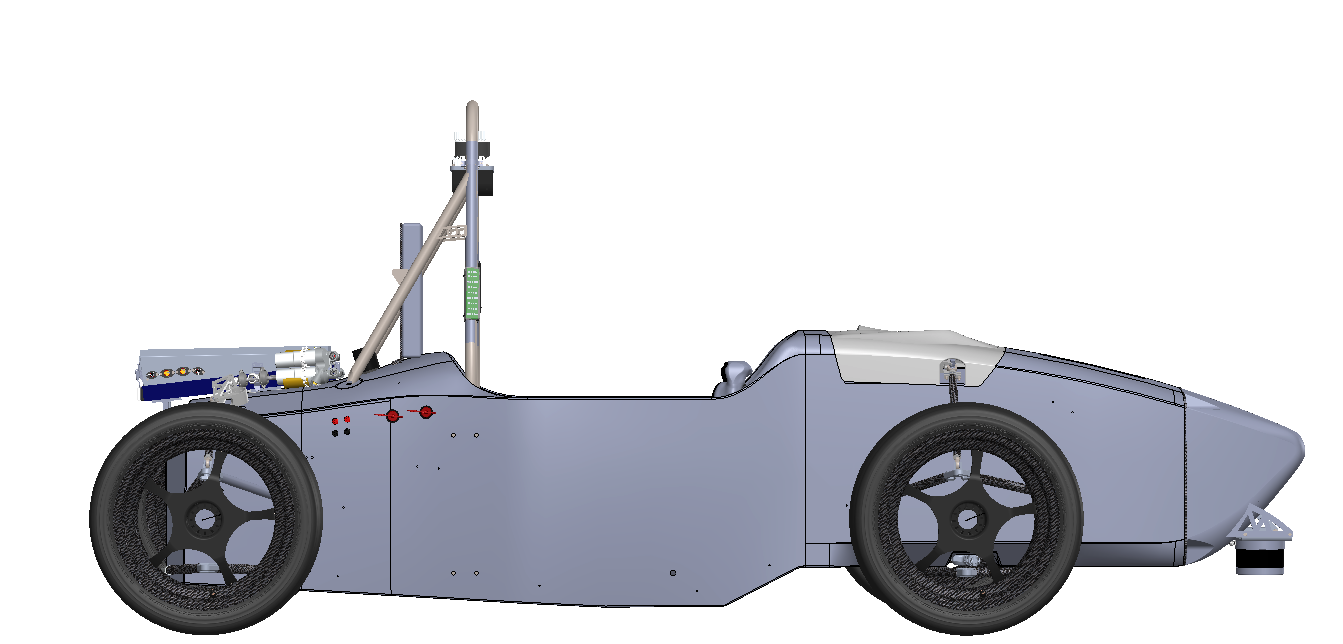
\includegraphics[width=0.8\linewidth]{0_Images/4_Implementation/LidarPlacements.png}
    \caption[Placement of the perception sensors.]
    {Placement of the perception sensors. A LiDAR and the camera are in the main hoop, while the other LiDAR is below the snout.}
    \label{Fig:SensorPlacements}
\end{figure}
\fi

\begin{figure}
    \centering
    
\includegraphics[width=0.8\linewidth]{0_Images/4_Implementation/SensorPlacements.eps}
    \caption[Placement of the perception sensors.]
    {Placement of the perception sensors. A LiDAR and the camera are in the main hoop, while the other LiDAR is below the snout.}
    \label{Fig:SensorPlacementsV2}
\end{figure}

\subsubsection{LiDAR detection algorithm}
The point cloud coming from the LiDARs get filtered based on position, where points too low, too high or too far away are discared. Then the ground is removed, by following the method used in \cite{GroundRemoval}. The point cloud is then downsampled into a voxel grid, and euclidian clustered, both using the PCL library \cite{PCL}. The true data in the downsampled clusters are then recreated and the centroid is found. Finally there is an outlier removal, where centroids with neighbors that are too close or too far away are removed. The centroids are then sent to the SLAM frontend as a set of detected cones.

\subsection{Camera}
For camera detection, a Basler PYTHON 1300 camera is placed in the main hoop(also shown in figure \ref{Fig:SensorPlacementsV2}), which is used for detection, as well as for determining the color of already detected cones. It has a 74.65 degree field of view and a resolution of 1280 x 1024, running at 200 Hz. \\

\subsubsection{Camera detection algorithm}
The images from the camera get fed into a neural net built on YOLO V3\cite{YOLOV3}. The last few layers of the net have been retrained on a quite extensive labeled dataset of cones, built up through the years by trading with other teams. This outputs bounding boxes on cones in the image, as well as the color of the detected cones. \\

The bounding boxes are then used to find the position in the body frame of the detected cones. Two methods have been tested for this. The first is using only geometry, considering the size and position of the bounding box. The second solution was to have the bounding boxes and the geometrically estimated positions sent into another neural net that corrects the initial estimate. This gave better results, the two errors in distance can be seen in figure \ref{Fig:rErrorCamera} and the error in angle in figure \ref{Fig:psiErrorCamera}.

\begin{figure}
    \centering
    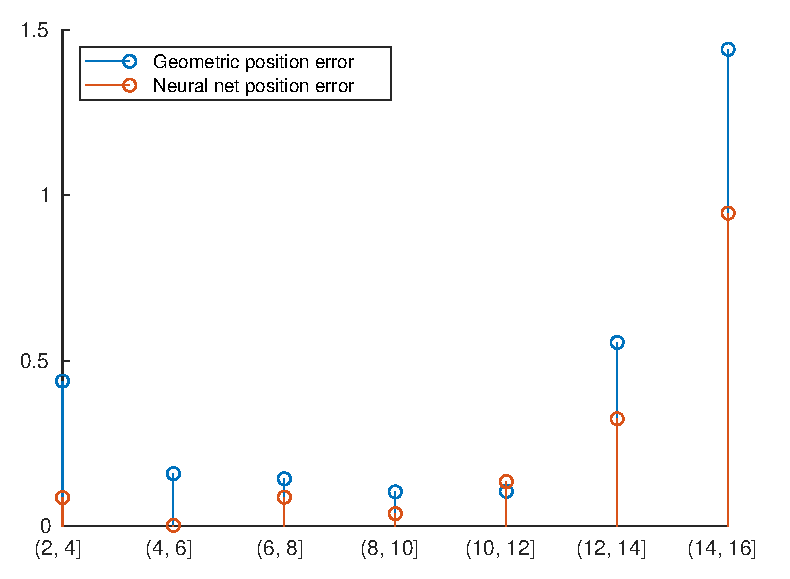
\includegraphics[width=0.8\linewidth]{0_Images/3_Theory/camDetection/rErrorCamera.eps}
    \caption[Error in the distance estimate of the two camera detection approaches.]
    {Error in the distance estimate of the two camera detection approaches.}
    \label{Fig:rErrorCamera}
\end{figure}

\begin{figure}
    \centering
    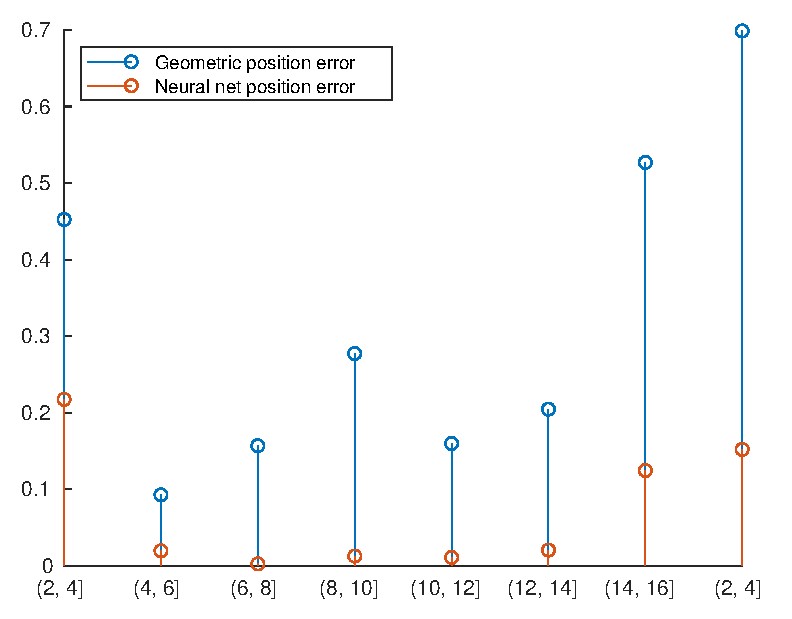
\includegraphics[width=0.8\linewidth]{0_Images/3_Theory/camDetection/psiErrorCamera.eps}
    \caption[Error in the angle estimate of the two camera detection approaches.]
    {Error in the angle estimate of the two camera detection approaches.}
    \label{Fig:psiErrorCamera}
\end{figure}

\subsection{INS}
The race car sports a Vectornav VN300 which is both an IMU as well as a GPS-receiver. It has a dual antenna setup where the two antennas are aligned with the x-axis of the car. This is done so it can get yaw angle, which the GPS gives out with 2 degrees of error. It outputs it's data at 400 Hz, and filters internally using a Kalman filter. \\ 

The INS outputs liner accelerations in 3 dimensions, the rate of change of the yaw, pitch and roll, as well as heading and a quite noisy position data from the GPS. \todo{Look over this, might want to rewrite whole subsection}

\subsection{Other}
Furthermore we have optical encoders giving us the RPM of each wheel. Another optical encoder measures steering wheel angle, which through a lookup table gives out the angle of the front wheels with the x-axis. There are also ride height sensors, that give the linear travel of the shock absorbers. This could indirectly give height above the ground, but in the authors opinion they are far from accurate enough to be usable.